% This must be in the first 5 lines to tell arXiv to use pdfLaTeX, which is strongly recommended.
\pdfoutput=1
% In particular, the hyperref package requires pdfLaTeX in order to break URLs across lines.
\documentclass[9pt]{article}

% Remove the "review" option to generate the final version.

\usepackage{multicol}
\usepackage{caption}
\usepackage[left=2cm,right=2cm,top=2cm,bottom=2.5cm]{geometry}
\usepackage[final]{naacl2021}
\usepackage{hyperref}
\usepackage{url}
\usepackage{amsmath}
\usepackage{graphicx}
\usepackage{amssymb}
\usepackage{hyperref}
\usepackage{subfig}
\hypersetup{
	colorlinks=true,
	linkcolor=blue,
	filecolor=magenta,      
	urlcolor=blue,
}

\usepackage{listings}
\usepackage{color}

\lstset{frame=tb,
	language=Java,
	aboveskip=3mm,
	belowskip=3mm,
	showstringspaces=false,
	columns=flexible,
	basicstyle={\small\ttfamily},
	numbers=none,
	breaklines=true,
	breakatwhitespace=true,
	tabsize=3
}

\definecolor{applegreen}{rgb}{0.55, 0.71, 0.0}
\definecolor{azure(colorwheel)}{rgb}{0.0, 0.5, 1.0}
\definecolor{awesome}{rgb}{1.0, 0.13, 0.32}
\definecolor{ao(english)}{rgb}{0.0, 0.5, 0.0}
\definecolor{darkmidnightblue}{rgb}{0.0, 0.2, 0.4}
% Standard package includes
\usepackage{times}
\usepackage{latexsym}

% For proper rendering and hyphenation of words containing Latin characters (including in bib files)
\usepackage[T1]{fontenc}
% For Vietnamese characters
% \usepackage[T5]{fontenc}
% See https://www.latex-project.org/help/documentation/encguide.pdf for other character sets

% This assumes your files are encoded as UTF8
\usepackage[utf8]{inputenc}

% This is not strictly necessary, and may be commented out,
% but it will improve the layout of the manuscript,
% and will typically save some space.
\usepackage{microtype}

% If the title and author information does not fit in the area allocated, uncomment the following
%
%\setlength\titlebox{<dim>}
%
% and set <dim> to something 5cm or larger.

\title{Instructions for NAACL-HLT 2021 Proceedings}

% Author information can be set in various styles:
% For several authors from the same institution:
% \author{Author 1 \and ... \and Author n \\
%         Address line \\ ... \\ Address line}
% if the names do not fit well on one line use
%         Author 1 \\ {\bf Author 2} \\ ... \\ {\bf Author n} \\
% For authors from different institutions:
% \author{Author 1 \\ Address line \\  ... \\ Address line
%         \And  ... \And
%         Author n \\ Address line \\ ... \\ Address line}
% To start a seperate ``row'' of authors use \AND, as in
% \author{Author 1 \\ Address line \\  ... \\ Address line
%         \AND
%         Author 2 \\ Address line \\ ... \\ Address line \And
%         Author 3 \\ Address line \\ ... \\ Address line}

\author{First Author \\
  Affiliation / Address line 1 \\
  Affiliation / Address line 2 \\
  Affiliation / Address line 3 \\
  \texttt{email@domain} \\\And
  Second Author \\
  Affiliation / Address line 1 \\
  Affiliation / Address line 2 \\
  Affiliation / Address line 3 \\
  \texttt{email@domain} \\}

\begin{document}
\maketitle
\begin{abstract}
Debloating Abstract
\end{abstract}

\section{Introduction}
Introduction


\section{Tools}
Explanation of all tools 

\subsection{CHISEL}
\paragraph{}
The input to the \textbf{CHISEL} tool is a C/C++ source file (test.c) which is to be debloated. Along with the source file , we give a specialized script which contains the high level specification of the desired output. The CHISEL tool then generates binary of the source code(test.c.chisel.c). Both the source and debloated program are then compiled by g++ or any other compiler and the binaries generated by the compiler are given to the ROP gadgets or Gadget Set Analyser(GSA) . The ROP gadget outputs the count of the  gadgets before and after debloating respectively.

\paragraph{}
CHISEL works on the Delta Debugging algorithm.The delta debugging algorithm optimizes the global functions calls,etc. first and then further approach local level reduction for the optimization. The process is continued till 1-minimal of a program is reached. Delta debugging ensures that there is no scope for further debloating.

\paragraph{}
Markov Decision Process for delta debugging is deployed to build a statistical model to get 1-minimal solution with lesser number of iterations than delta debugging alone.

\subsection{INST2VEC}
\paragraph{}
Inst2vec  is the technique of processing the source code into the features vector for modeling the Reinforcement Learning. It follows an approach similar to skip-gram model in Natural Language Processing of pre-defined context size. The source code is first compiled into LLVM IR code. The LLVM IR is in the form of a static single assignment.As LLVM IR  is independent of machine or hardware architecture and programming language , it becomes easy to train the program embeddings.The approach is similar to word2vec model.

\paragraph{}
With the LLVM IR , the contextual flow graph (XFG)is created. XFG takes into account both the data flow and control flow of the program. With these XFGs generated from LLVM IR , the consecutive statement pairs are made of pre-defined context size . These statement pairs are then  checked for duplication. The XFGs pairs are made by constructing a dual graph with statement as nodes and removing duplicate edges. The process is then followed by removing statements of negligible presence. We get an inst2vec after subsampling of frequent pairs which can be optimized and trained. XFGs ensures that the semantics of statements are preserved.

\subsection{TRIMMER}
\paragraph{}
The source code is converted to LLVM IR  and given as an input to the trimmer tool along with the manifest file consisting of user defined configuration. The TRIMMER first performs input specialization with respect to the user defined configuration . The second part is loop unrolling . The loop unrolling becomes important step to make interprocedural constant propagation easier. Constant Propagation is the final stage in the tool. The specialized code processed by the TRIMMER is then given as input to the linker . The linker also reads the linker flags from the manifest file and generates a final specialized binary executable file.


\section{Overview}

How these tools solve debloating
\begin{quote}
\begin{verbatim}
\documentclass[11pt]{article}
\end{verbatim}
\end{quote}


\section{Setup}
Setup for running the pipelines. 

\subsection{Aim}
Footnotes are inserted with the \verb|\footnote| command.\footnote{This is a footnote.}

\subsection{Tables and figures}

See Table~\ref{tab:accents} for an example of a table and its caption.
\textbf{Do not override the default caption sizes.}

\begin{figure*}
\begin{multicols}{4}[\columnsep=1cm]
    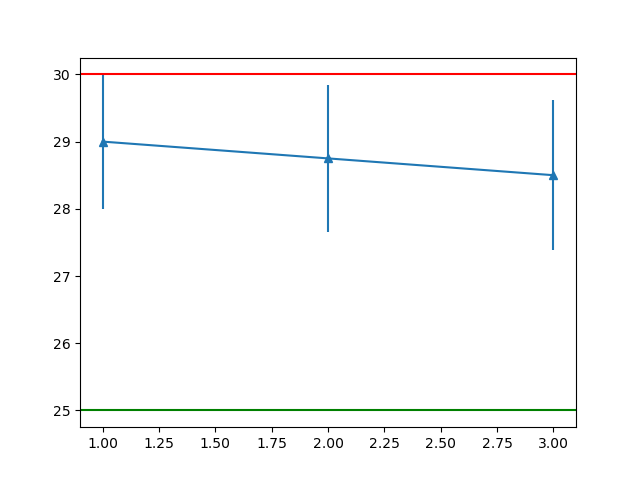
\includegraphics[width=\linewidth]{b}
    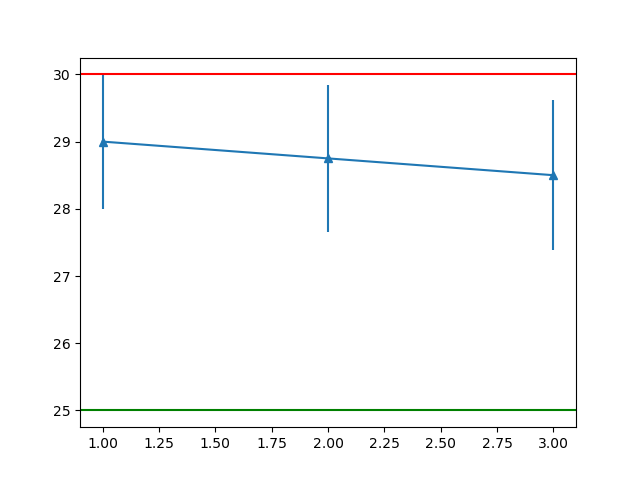
\includegraphics[width=\linewidth]{b}
    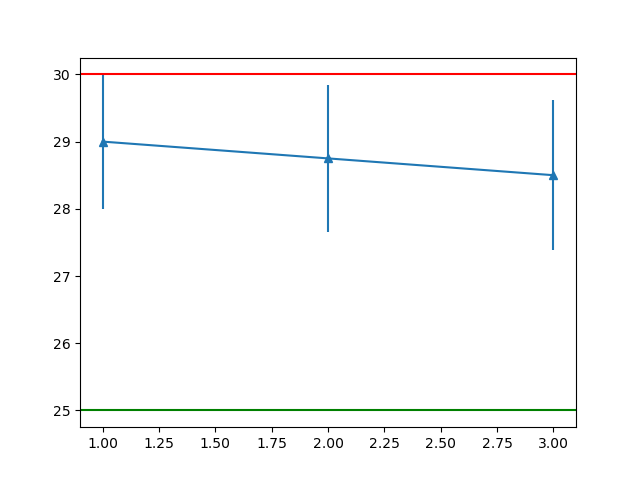
\includegraphics[width=\linewidth]{b}
    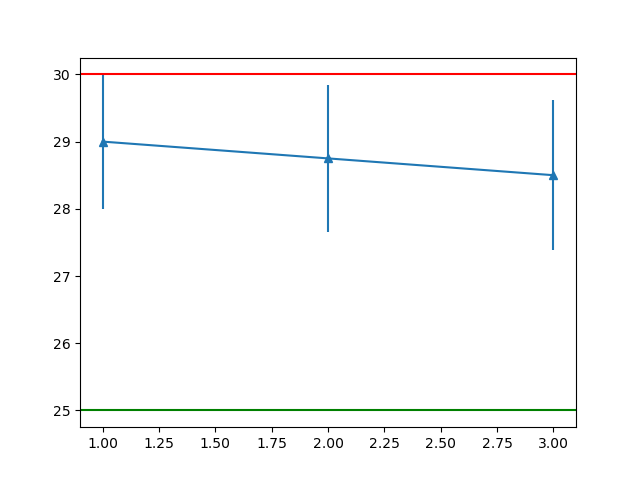
\includegraphics[width=\linewidth]{b}
    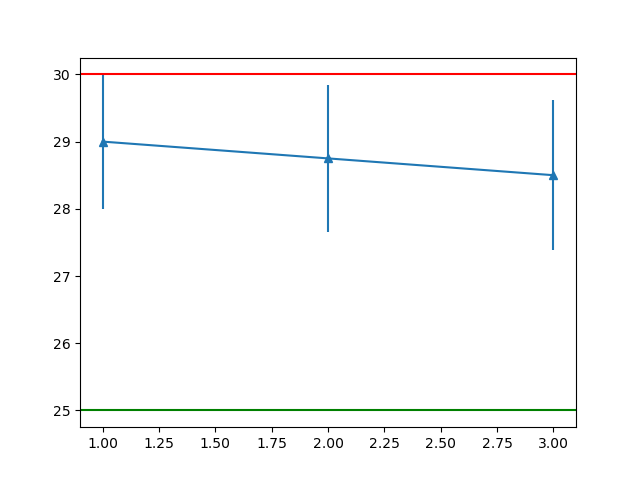
\includegraphics[width=\linewidth]{b}
    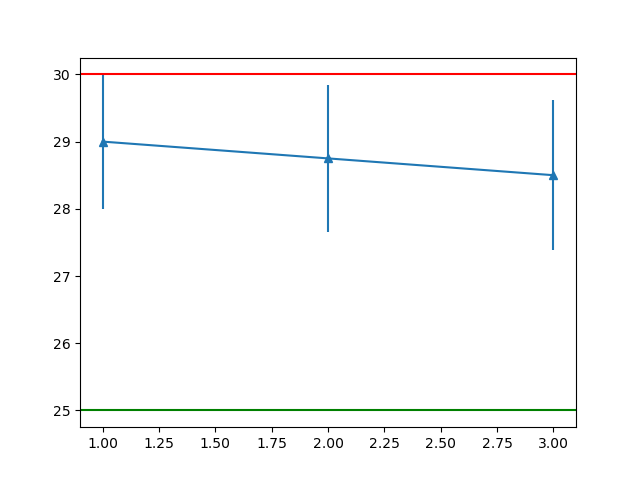
\includegraphics[width=\linewidth]{b}
    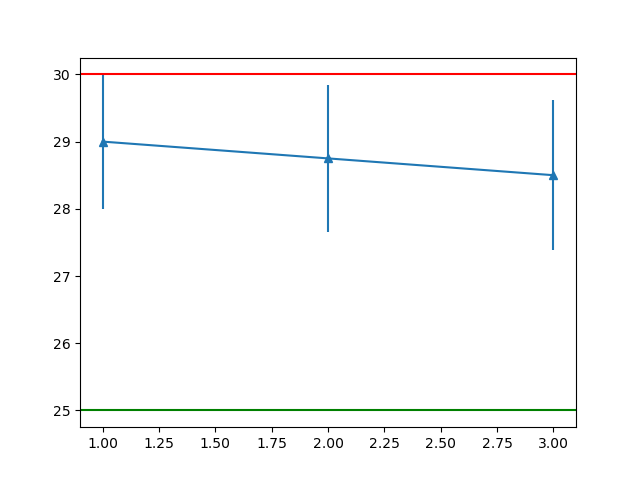
\includegraphics[width=\linewidth]{b}
    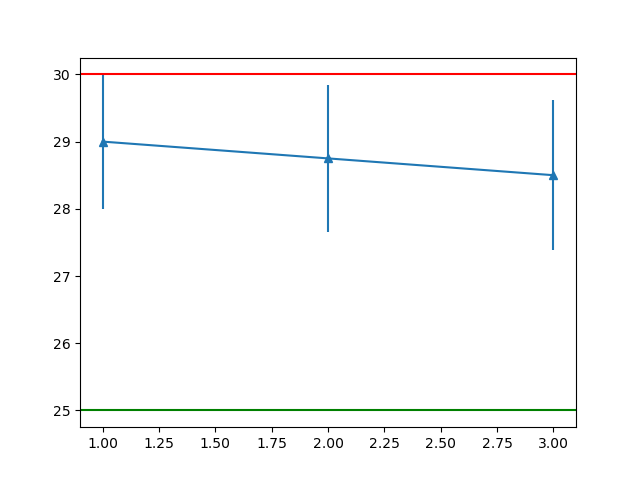
\includegraphics[width=\linewidth]{b}
    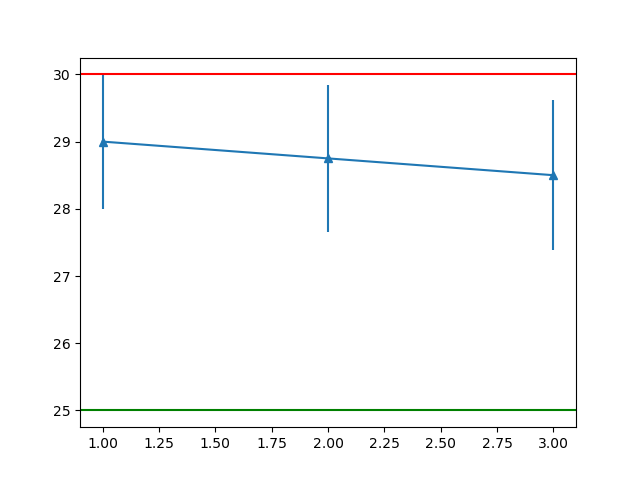
\includegraphics[width=\linewidth]{b}
    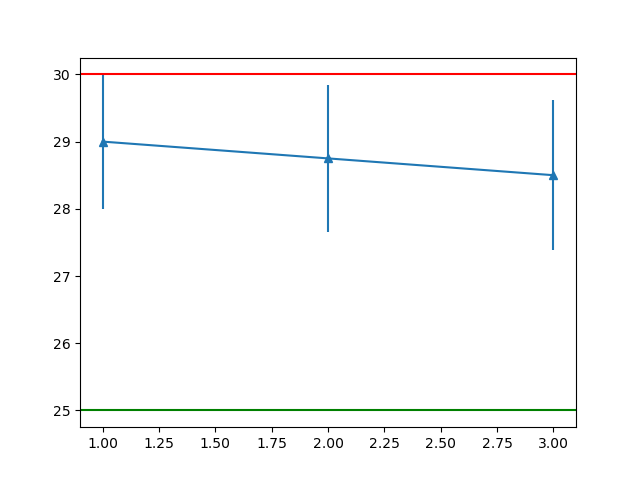
\includegraphics[width=\linewidth]{b}
    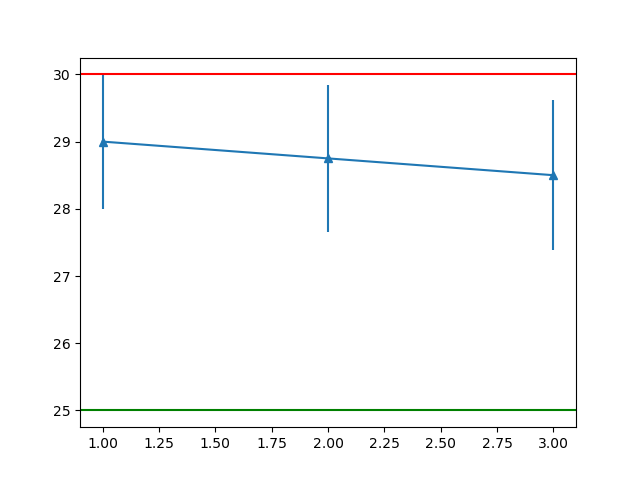
\includegraphics[width=\linewidth]{b}
    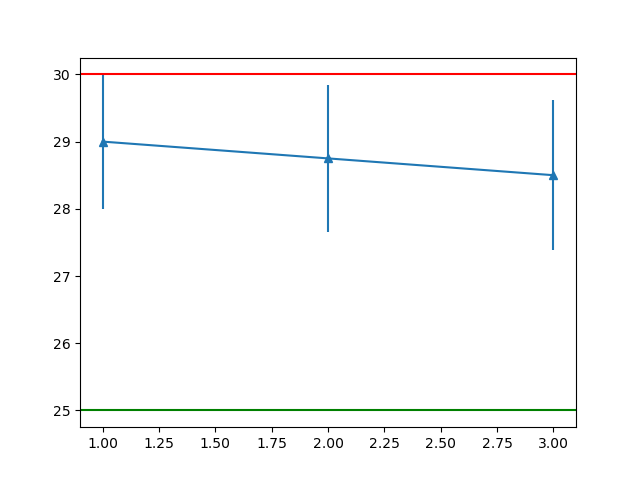
\includegraphics[width=\linewidth]{b}
    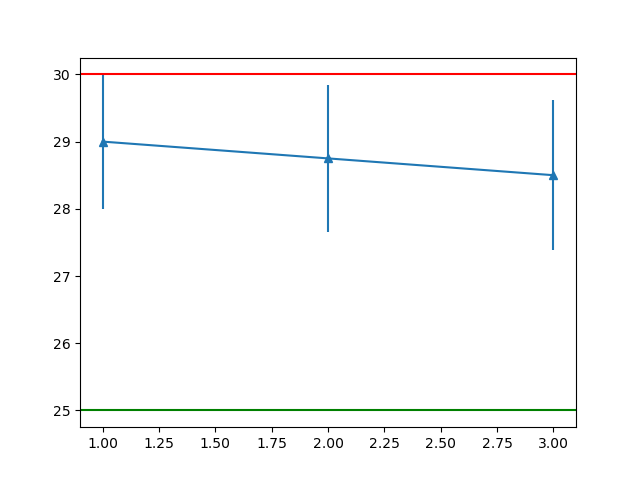
\includegraphics[width=\linewidth]{b}
    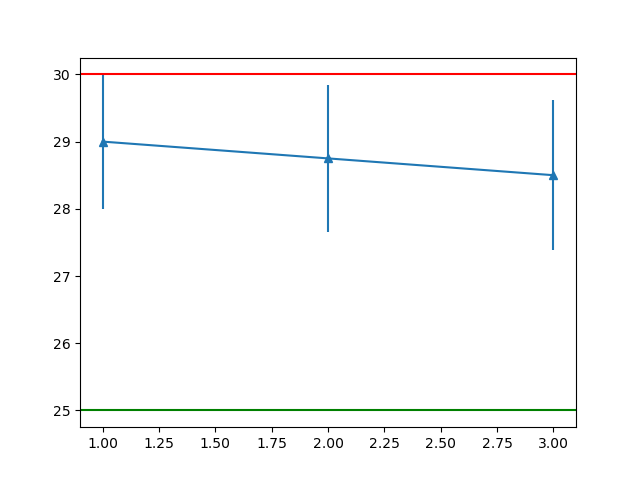
\includegraphics[width=\linewidth]{b}
    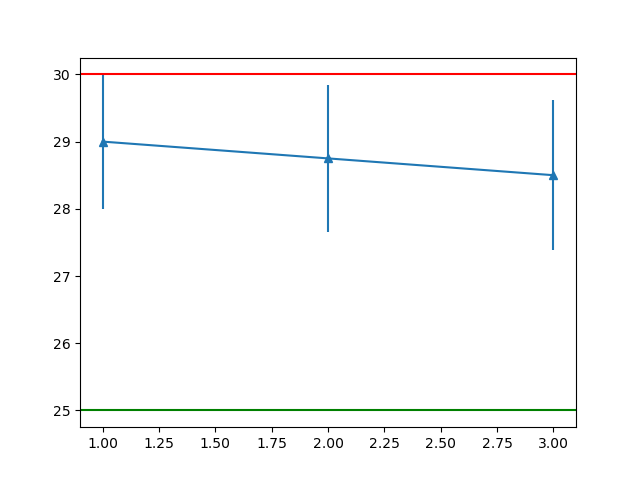
\includegraphics[width=\linewidth]{b}
    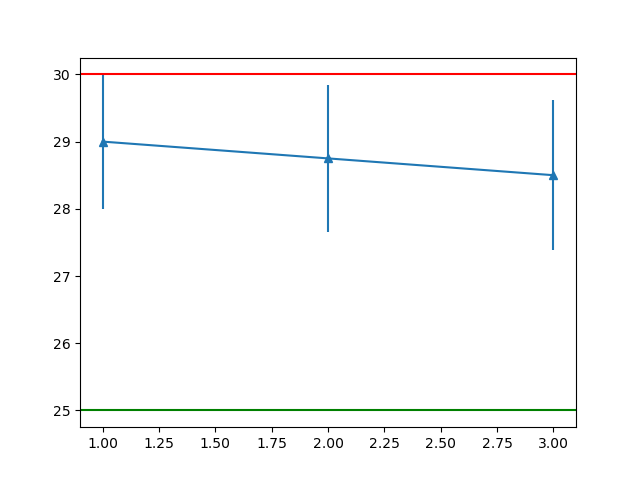
\includegraphics[width=\linewidth]{b}
    %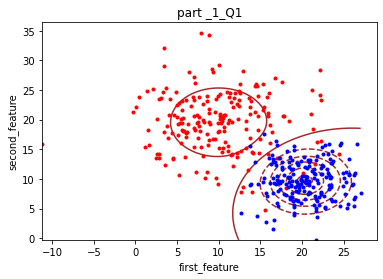
\includegraphics[width=\linewidth]{a}\par 
    \end{multicols}
    %\caption{caption here}  Uncomment if caption needed
    
Write the description here. Dummy description .Write the description here. Dummy description Write the description here. Dummy description Write the description here. Dummy description Write the description here. Dummy description Write the description here. Dummy description Write the description here. Dummy description Write the description here. Dummy description Write the description here. Dummy description Write the description here. Dummy description Write the description here. Dummy description Write the description here. Dummy description Write the description here. Dummy description.
\begin{multicols}{2}
    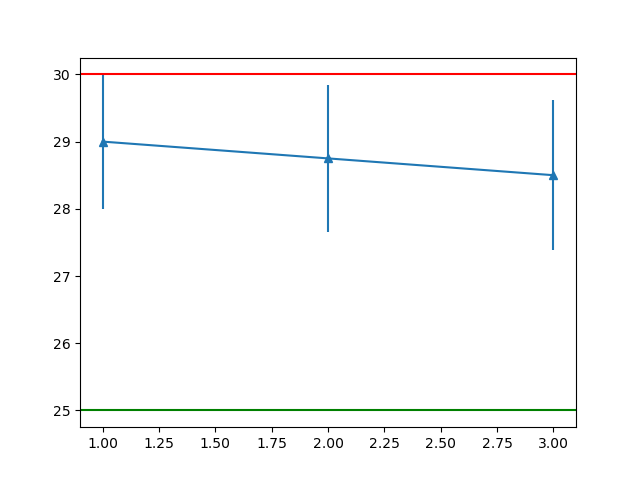
\includegraphics[width=\linewidth,scale=0.5]{b}
    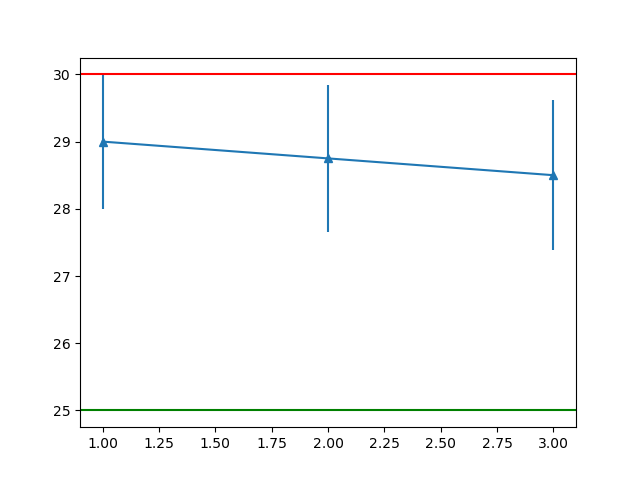
\includegraphics[width=\linewidth,scale=0.5]{b}
    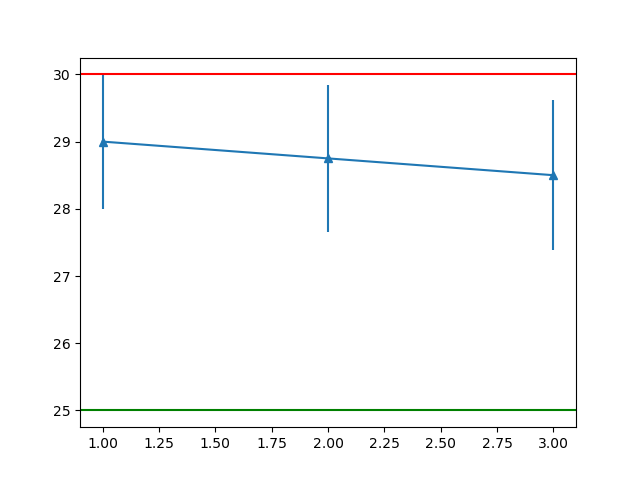
\includegraphics[width=\linewidth,scale=0.5]{b}
    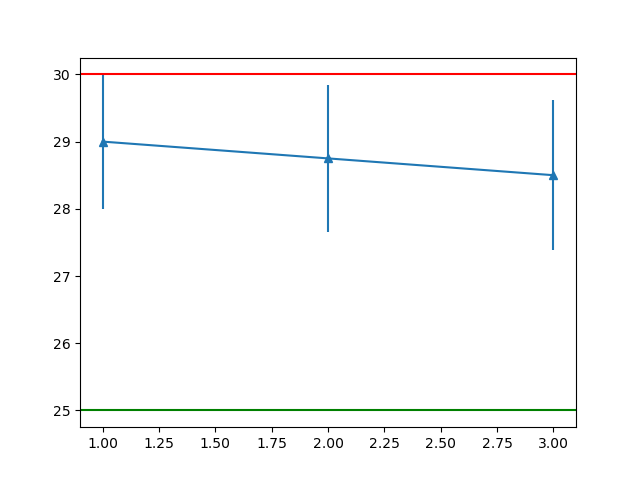
\includegraphics[width=\linewidth,scale=0.5]{b}
    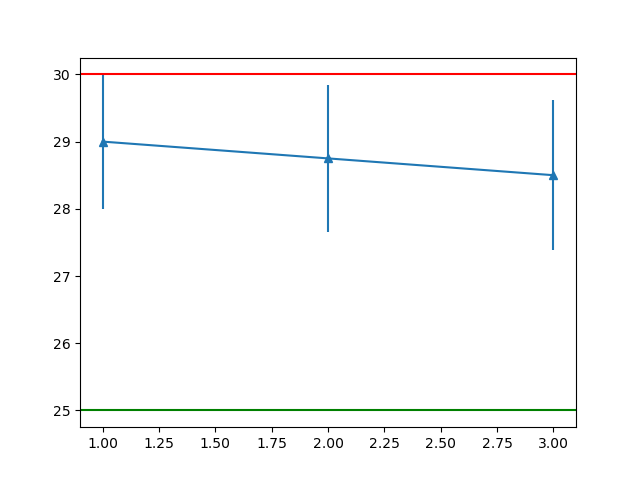
\includegraphics[width=\linewidth,scale=0.5]{b}
    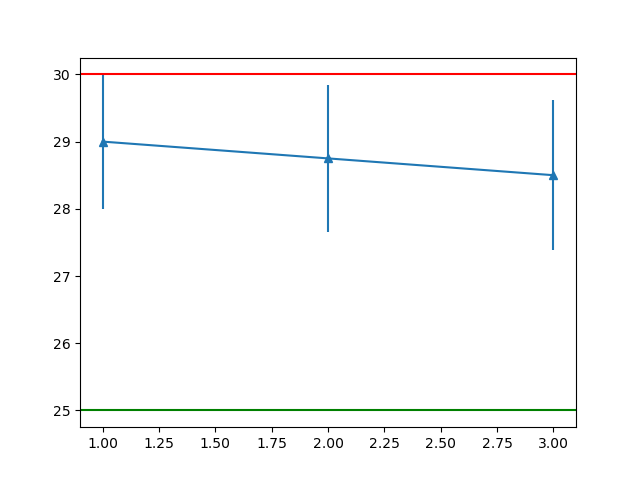
\includegraphics[width=\linewidth,scale=0.5]{b}
    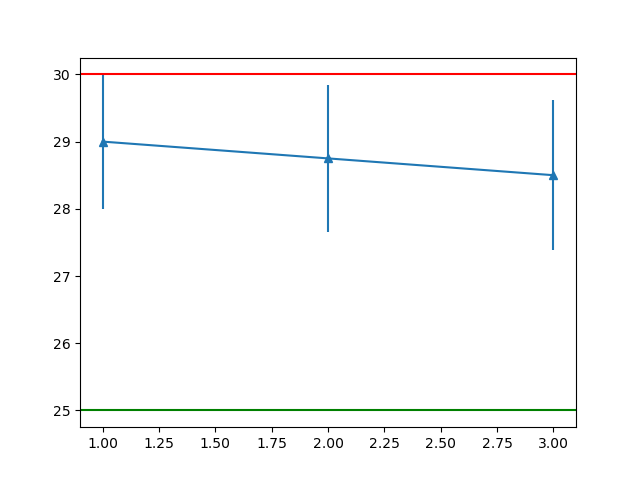
\includegraphics[width=\linewidth,scale=0.5]{b}
    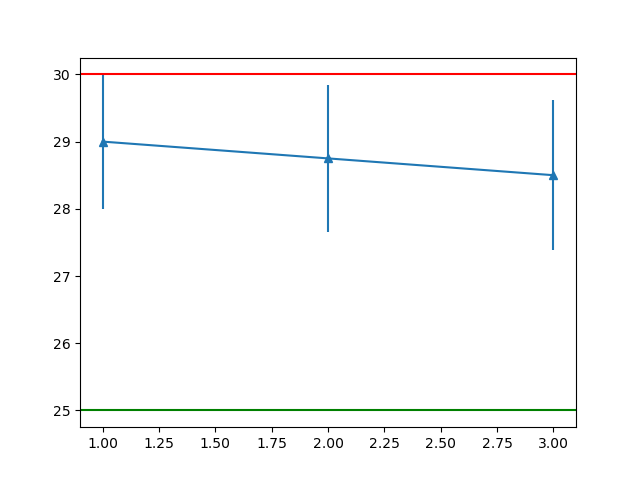
\includegraphics[width=\linewidth,scale=0.5]{b}
\end{multicols}
%getting problem here
Write the description here. Dummy description .Write the description here. Dummy description Write the description here. Dummy description Write the description here. Dummy description Write the description here. Dummy description Write the description here. Dummy description Write the description here. Dummy description Write the description here. Dummy description Write the description here. Dummy description Write the description here. Dummy description Write the description here. Dummy description Write the description here. Dummy description Write the description here. Dummy description.

\end{figure*}



%\begin{multicols}{3}[\columnsep=3cm]
%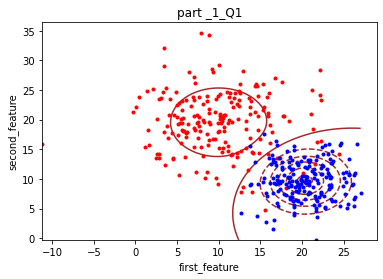
\includegraphics[scale=0.3]{a}
%\columnbreak
%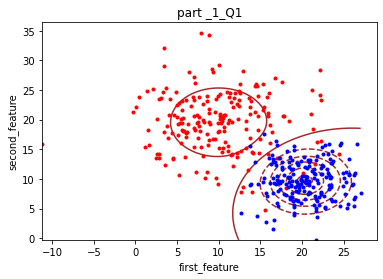
\includegraphics[scale=0.3]{a}
%\columnbreak
%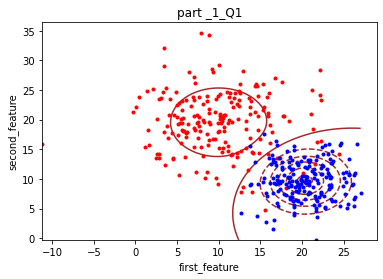
\includegraphics[scale=0.3]{a}
%\end{multicols}




\begin{table}
\centering
\begin{tabular}{lc}
\hline
\textbf{Command} & \textbf{Output}\\
\hline
\verb|{\"a}| & {\"a} \\
\verb|{\^e}| & {\^e} \\
\verb|{\`i}| & {\`i} \\ 
\verb|{\.I}| & {\.I} \\ 
\verb|{\o}| & {\o} \\
\verb|{\'u}| & {\'u}  \\ 
\verb|{\aa}| & {\aa}  \\\hline
\end{tabular}
\begin{tabular}{lc}
\hline
\textbf{Command} & \textbf{Output}\\
\hline
\verb|{\c c}| & {\c c} \\ 
\verb|{\u g}| & {\u g} \\ 
\verb|{\l}| & {\l} \\ 
\verb|{\~n}| & {\~n} \\ 
\verb|{\H o}| & {\H o} \\ 
\verb|{\v r}| & {\v r} \\ 
\verb|{\ss}| & {\ss} \\
\hline
\end{tabular}
\caption{Example commands for accented characters, to be used in, \emph{e.g.}, Bib\TeX{} entries.}
\label{tab:accents}
\end{table}

\subsection{Observations}

Users of older versions of \LaTeX{} may encounter the following error during compilation: 
\begin{quote}
\tt\verb|\pdfendlink| ended up in different nesting level than \verb|\pdfstartlink|.
\end{quote}
This happens when pdf\LaTeX{} is used and a citation splits across a page boundary. The best way to fix this is to upgrade \LaTeX{} to 2018-12-01 or later.

\subsection{Inferences}

\begin{table*}
\centering
\begin{tabular}{lll}
\hline
\textbf{Output} & \textbf{natbib command} & \textbf{Old ACL-style command}\\
\hline
\citep{Gusfield:97} & \verb|\citep| & \verb|\cite| \\
\citealp{Gusfield:97} & \verb|\citealp| & no equivalent \\
\citet{Gusfield:97} & \verb|\citet| & \verb|\newcite| \\
\citeyearpar{Gusfield:97} & \verb|\citeyearpar| & \verb|\shortcite| \\
\hline
\end{tabular}
\caption{\label{citation-guide}
Citation commands supported by the style file.
The style is based on the natbib package and supports all natbib citation commands.
It also supports commands defined in previous ACL style files for compatibility.
}
\end{table*}

Table~\ref{citation-guide} shows the syntax supported by the style files.
We encourage you to use the natbib styles.
You can use the command \verb|\citet| (cite in text) to get ``author (year)'' citations, like this citation to a paper by \citet{Gusfield:97}.
You can use the command \verb|\citep| (cite in parentheses) to get ``(author, year)'' citations \citep{Gusfield:97}.
You can use the command \verb|\citealp| (alternative cite without parentheses) to get ``author, year'' citations, which is useful for using citations within parentheses (e.g. \citealp{Gusfield:97}).

\subsection{Failures}

\nocite{Ando2005,borschinger-johnson-2011-particle,andrew2007scalable,rasooli-tetrault-2015,goodman-etal-2016-noise,harper-2014-learning}

The \LaTeX{} and Bib\TeX{} style files provided roughly follow the American Psychological Association format.
If your own bib file is named \texttt{custom.bib}, then placing the following before any appendices in your \LaTeX{} file will generate the references section for you:
\begin{quote}
\begin{verbatim}
\bibliographystyle{acl_natbib}
\bibliography{custom}
\end{verbatim}
\end{quote}

You can obtain the complete ACL Anthology as a Bib\TeX{} file from \url{https://aclweb.org/anthology/anthology.bib.gz}.
To include both the Anthology and your own .bib file, use the following instead of the above.
\begin{quote}
\begin{verbatim}
\bibliographystyle{acl_natbib}
\bibliography{anthology,custom}
\end{verbatim}
\end{quote}

Please see Section~\ref{sec:bibtex} for information on preparing Bib\TeX{} files.

\subsection{Future Runs}

See Appendix~\ref{sec:appendix} for more artifacts

\section{Final Result}
\label{sec:bibtex}


\section{Comparision Insights}

\begin{figure}%
	\centering
	\subfloat[\centering OOCAM Run : \textbf{\texttt{bzip2}}]{{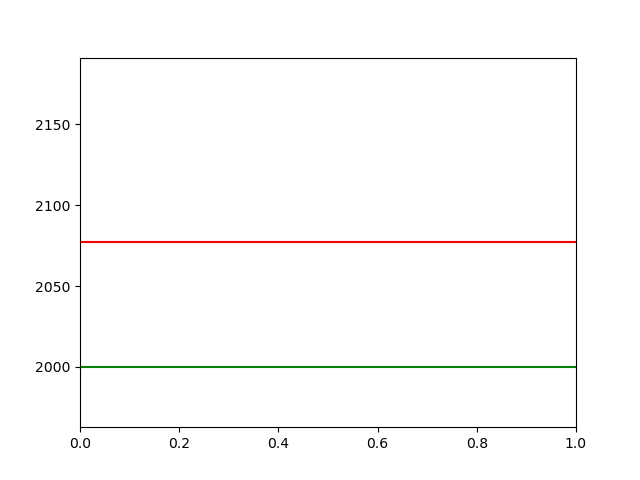
\includegraphics[width=6cm]{occam_graph_5_10.png} }}%
	\qquad
	\subfloat[\centering OOCAM Run : \textbf{\texttt{module}} example]{{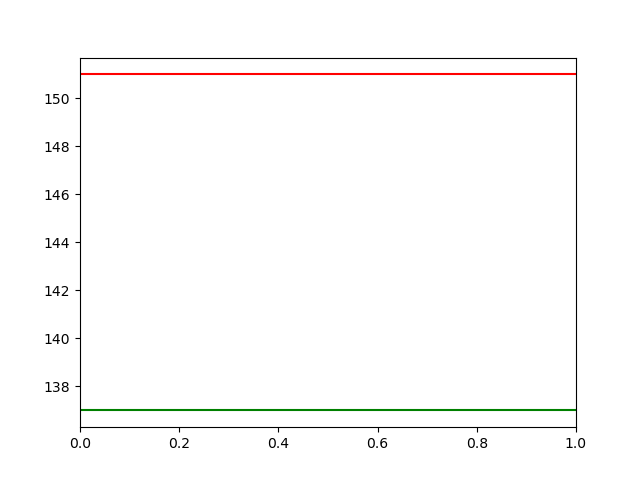
\includegraphics[width=6cm]{occam_graph_4_10.png} }}%
	\caption{OCCAM Tool runs on \textbf{\texttt{bzip2}} \& \textbf{\texttt{module}}. \textbf{\color{red} Before} and \textbf{\color{ao(english)} After} debloating}%
	\subfloat[\centering OOCAM Run : \textbf{\texttt{bzip2}}]{{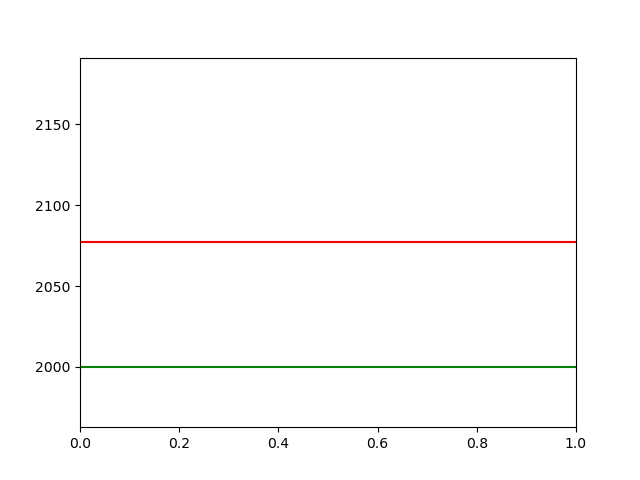
\includegraphics[width=6cm]{occam_graph_5_10.png} }}%
	\qquad
	\subfloat[\centering OOCAM Run : \textbf{\texttt{module}} example]{{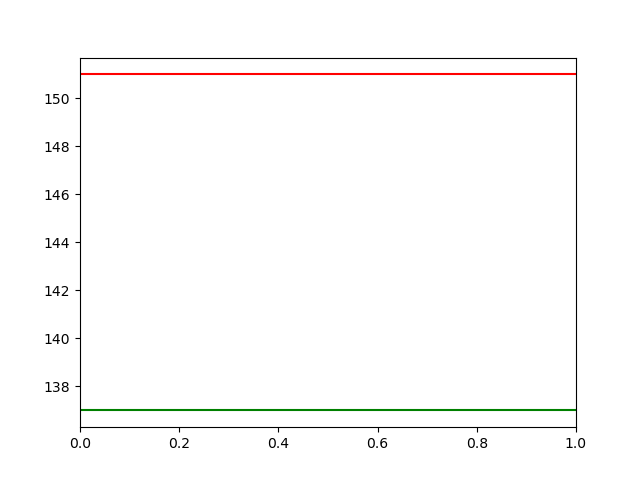
\includegraphics[width=6cm]{occam_graph_4_10.png} }}%
	\caption{OCCAM Tool runs on \textbf{\texttt{bzip2}} \& \textbf{\texttt{module}}. \textbf{\color{red} Before} and \textbf{\color{ao(english)} After} debloating}%
	\label{fig:example3}%
\end{figure}

\begin{figure}%
	\centering
	\subfloat[\centering OOCAM Run : \textbf{\texttt{bzip2}}]{{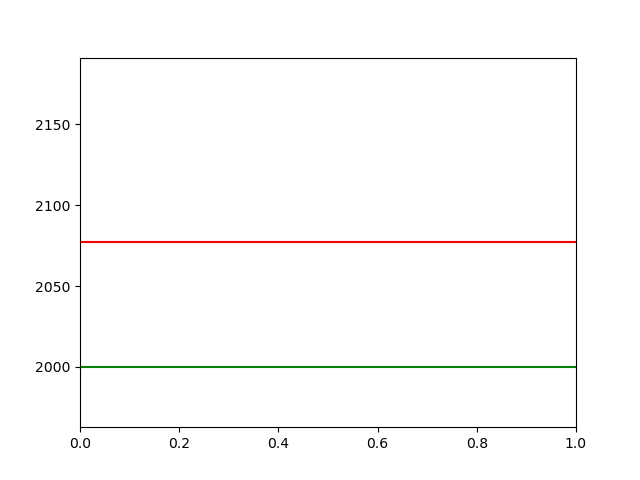
\includegraphics[width=6cm]{occam_graph_5_10.png} }}%
	\qquad
	\subfloat[\centering OOCAM Run : \textbf{\texttt{module}} example]{{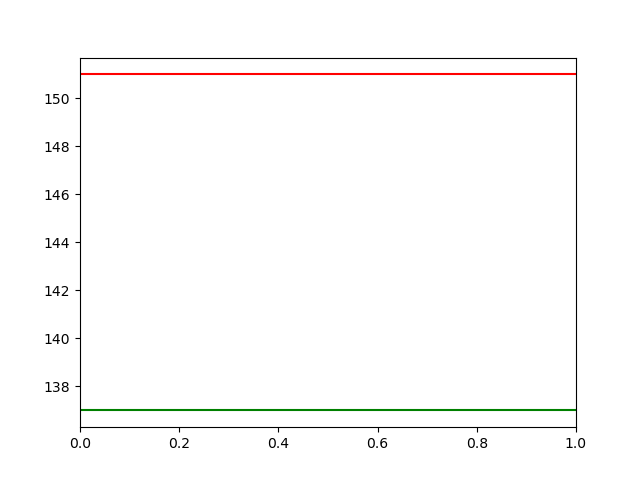
\includegraphics[width=6cm]{occam_graph_4_10.png} }}%
	\caption{OCCAM Tool runs on \textbf{\texttt{bzip2}} \& \textbf{\texttt{module}}. \textbf{\color{red} Before} and \textbf{\color{ao(english)} After} debloating}%
	\subfloat[\centering OOCAM Run : \textbf{\texttt{bzip2}}]{{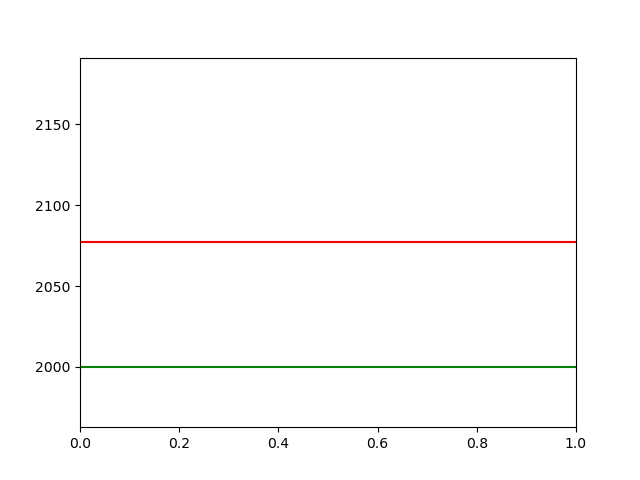
\includegraphics[width=6cm]{occam_graph_5_10.png} }}%
	\qquad
	\subfloat[\centering OOCAM Run : \textbf{\texttt{module}} example]{{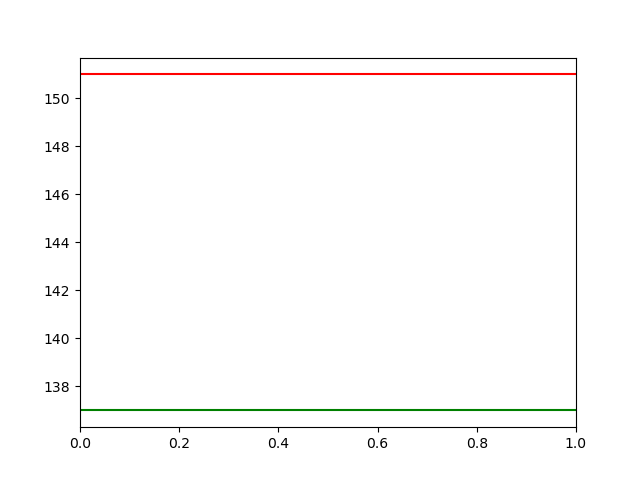
\includegraphics[width=6cm]{occam_graph_4_10.png} }}%
	\caption{OCCAM Tool runs on \textbf{\texttt{bzip2}} \& \textbf{\texttt{module}}. \textbf{\color{red} Before} and \textbf{\color{ao(english)} After} debloating}%
	\label{fig:example3}%
\end{figure}

\section{Comparision Insights}

\begin{figure}%
	\centering
	\subfloat[\centering OOCAM Run : \textbf{\texttt{bzip2}}]{{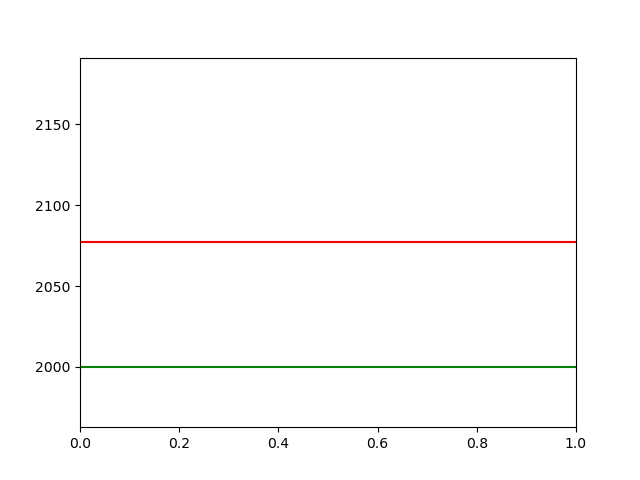
\includegraphics[width=6cm]{occam_graph_5_10.png} }}%
	\qquad
	\subfloat[\centering OOCAM Run : \textbf{\texttt{module}} example]{{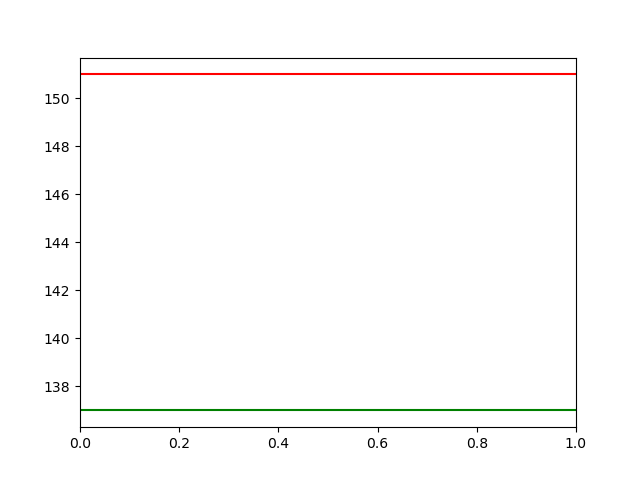
\includegraphics[width=6cm]{occam_graph_4_10.png} }}%
	\caption{OCCAM Tool runs on \textbf{\texttt{bzip2}} \& \textbf{\texttt{module}}. \textbf{\color{red} Before} and \textbf{\color{ao(english)} After} debloating}%
	\subfloat[\centering OOCAM Run : \textbf{\texttt{bzip2}}]{{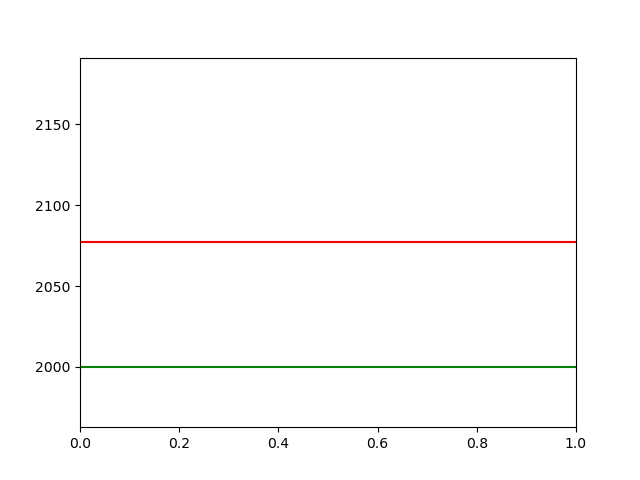
\includegraphics[width=6cm]{occam_graph_5_10.png} }}%
	\qquad
	\subfloat[\centering OOCAM Run : \textbf{\texttt{module}} example]{{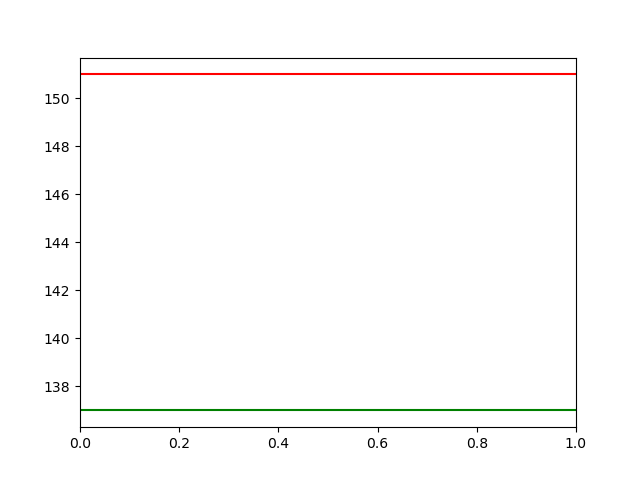
\includegraphics[width=6cm]{occam_graph_4_10.png} }}%
	\caption{OCCAM Tool runs on \textbf{\texttt{bzip2}} \& \textbf{\texttt{module}}. \textbf{\color{red} Before} and \textbf{\color{ao(english)} After} debloating}%
	\label{fig:example3}%
\end{figure}

\begin{figure}%
	\centering
	\subfloat[\centering OOCAM Run : \textbf{\texttt{bzip2}}]{{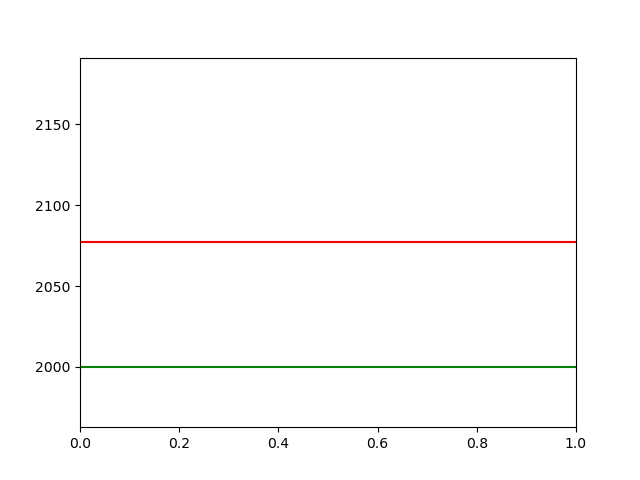
\includegraphics[width=6cm]{occam_graph_5_10.png} }}%
	\qquad
	\subfloat[\centering OOCAM Run : \textbf{\texttt{module}} example]{{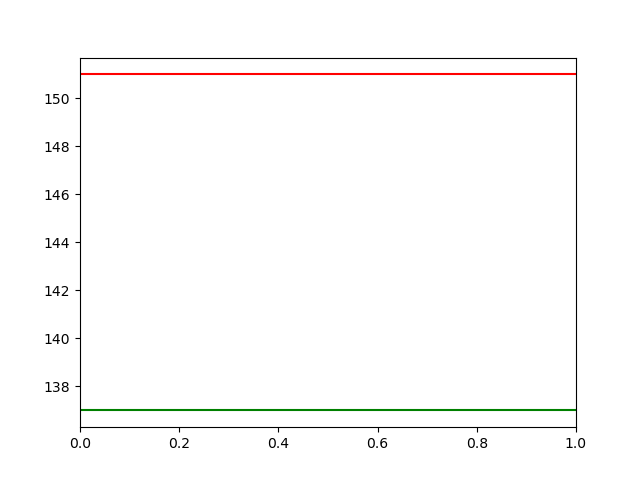
\includegraphics[width=6cm]{occam_graph_4_10.png} }}%
	\caption{OCCAM Tool runs on \textbf{\texttt{bzip2}} \& \textbf{\texttt{module}}. \textbf{\color{red} Before} and \textbf{\color{ao(english)} After} debloating}%
	\subfloat[\centering OOCAM Run : \textbf{\texttt{bzip2}}]{{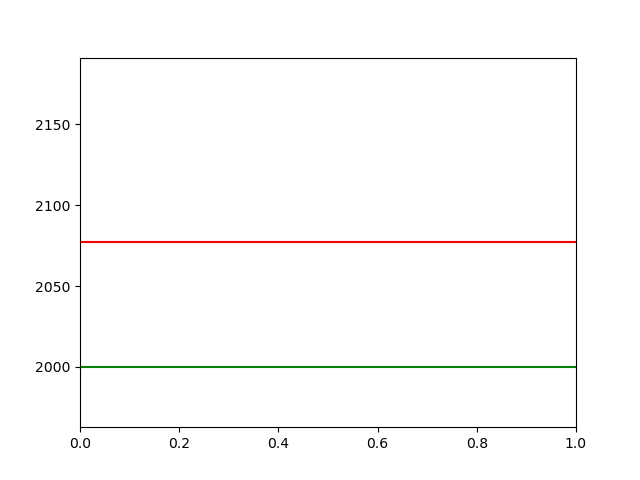
\includegraphics[width=6cm]{occam_graph_5_10.png} }}%
	\qquad
	\subfloat[\centering OOCAM Run : \textbf{\texttt{module}} example]{{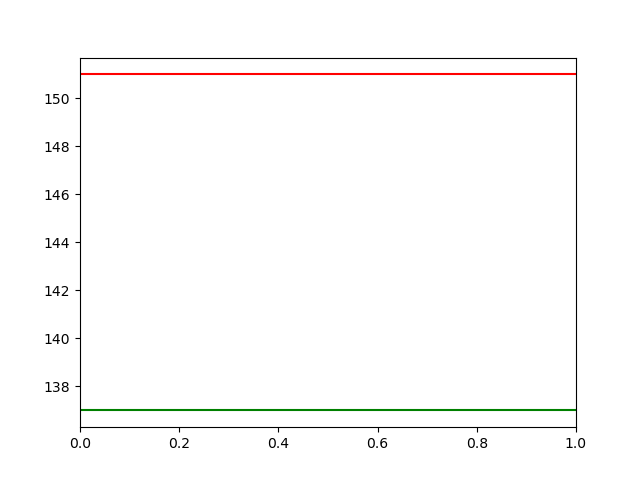
\includegraphics[width=6cm]{occam_graph_4_10.png} }}%
	\caption{OCCAM Tool runs on \textbf{\texttt{bzip2}} \& \textbf{\texttt{module}}. \textbf{\color{red} Before} and \textbf{\color{ao(english)} After} debloating}%
	\label{fig:example3}%
\end{figure}

\section{Comparision Insights}

\begin{figure}%
	\centering
	\subfloat[\centering OOCAM Run : \textbf{\texttt{bzip2}}]{{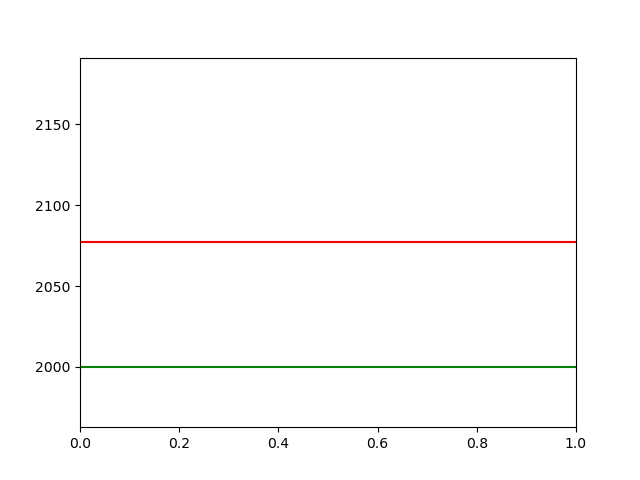
\includegraphics[width=6cm]{occam_graph_5_10.png} }}%
	\qquad
	\subfloat[\centering OOCAM Run : \textbf{\texttt{module}} example]{{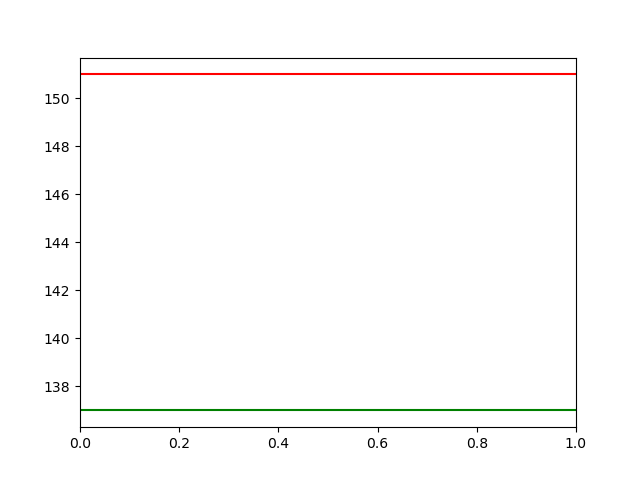
\includegraphics[width=6cm]{occam_graph_4_10.png} }}%
	\caption{OCCAM Tool runs on \textbf{\texttt{bzip2}} \& \textbf{\texttt{module}}. \textbf{\color{red} Before} and \textbf{\color{ao(english)} After} debloating}%
	\subfloat[\centering OOCAM Run : \textbf{\texttt{bzip2}}]{{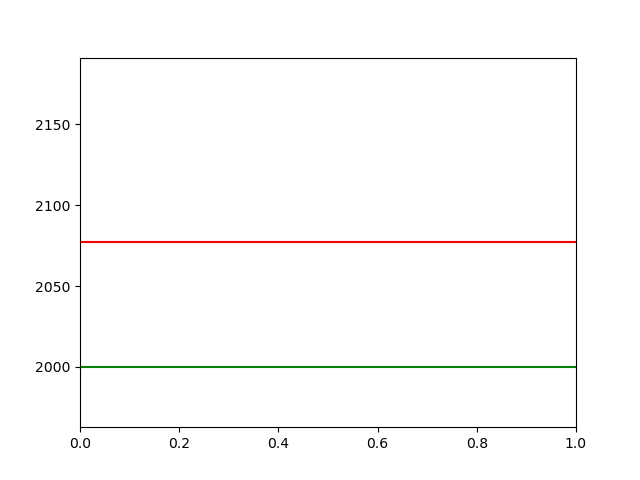
\includegraphics[width=6cm]{occam_graph_5_10.png} }}%
	\qquad
	\subfloat[\centering OOCAM Run : \textbf{\texttt{module}} example]{{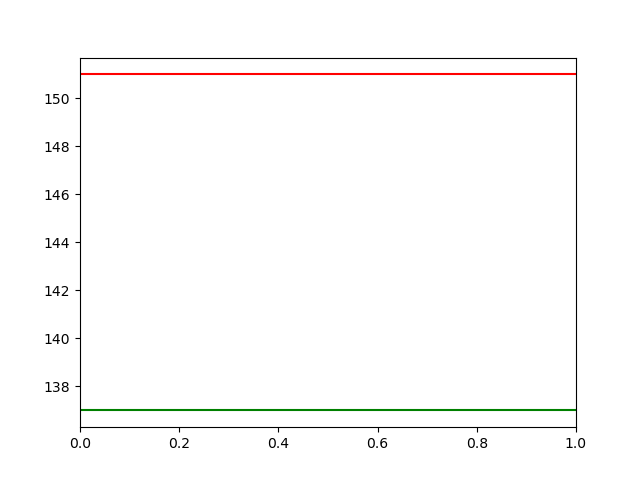
\includegraphics[width=6cm]{occam_graph_4_10.png} }}%
	\caption{OCCAM Tool runs on \textbf{\texttt{bzip2}} \& \textbf{\texttt{module}}. \textbf{\color{red} Before} and \textbf{\color{ao(english)} After} debloating}%
	\label{fig:example3}%
\end{figure}

\begin{figure}%
	\centering
	\subfloat[\centering OOCAM Run : \textbf{\texttt{bzip2}}]{{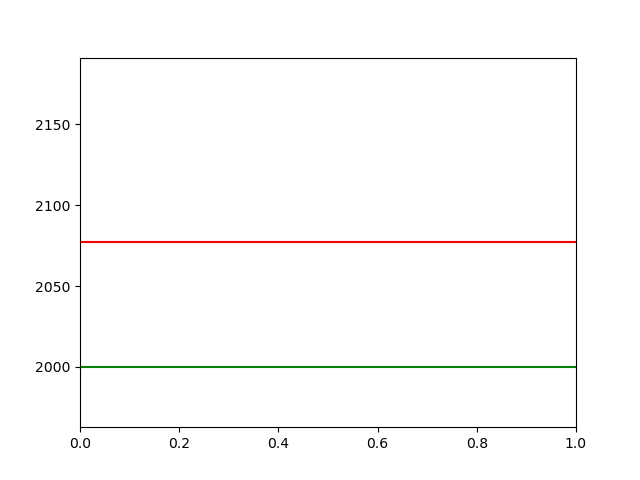
\includegraphics[width=6cm]{occam_graph_5_10.png} }}%
	\qquad
	\subfloat[\centering OOCAM Run : \textbf{\texttt{module}} example]{{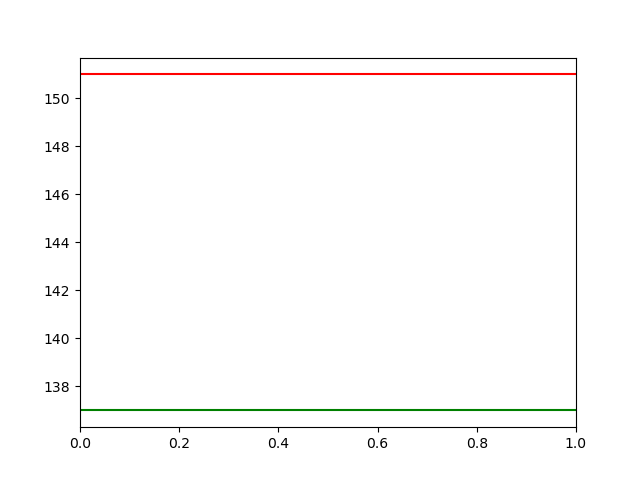
\includegraphics[width=6cm]{occam_graph_4_10.png} }}%
	\caption{OCCAM Tool runs on \textbf{\texttt{bzip2}} \& \textbf{\texttt{module}}. \textbf{\color{red} Before} and \textbf{\color{ao(english)} After} debloating}%
	\subfloat[\centering OOCAM Run : \textbf{\texttt{bzip2}}]{{\includegraphics[width=6cm]{occam_graph_5_10.png} }}%
	\qquad
	\subfloat[\centering OOCAM Run : \textbf{\texttt{module}} example]{{\includegraphics[width=6cm]{occam_graph_4_10.png} }}%
	\caption{OCCAM Tool runs on \textbf{\texttt{bzip2}} \& \textbf{\texttt{module}}. \textbf{\color{red} Before} and \textbf{\color{ao(english)} After} debloating}%
	\label{fig:example3}%
\end{figure}
\section{Comparision Insights}

\begin{figure}%
	\centering
	\subfloat[\centering OOCAM Run : \textbf{\texttt{bzip2}}]{{\includegraphics[width=6cm]{occam_graph_5_10.png} }}%
	\qquad
	\subfloat[\centering OOCAM Run : \textbf{\texttt{module}} example]{{\includegraphics[width=6cm]{occam_graph_4_10.png} }}%
	\caption{OCCAM Tool runs on \textbf{\texttt{bzip2}} \& \textbf{\texttt{module}}. \textbf{\color{red} Before} and \textbf{\color{ao(english)} After} debloating}%
	\subfloat[\centering OOCAM Run : \textbf{\texttt{bzip2}}]{{\includegraphics[width=6cm]{occam_graph_5_10.png} }}%
	\qquad
	\subfloat[\centering OOCAM Run : \textbf{\texttt{module}} example]{{\includegraphics[width=6cm]{occam_graph_4_10.png} }}%
	\caption{OCCAM Tool runs on \textbf{\texttt{bzip2}} \& \textbf{\texttt{module}}. \textbf{\color{red} Before} and \textbf{\color{ao(english)} After} debloating}%
	\label{fig:example3}%
\end{figure}

\begin{figure}%
	\centering
	\subfloat[\centering OOCAM Run : \textbf{\texttt{bzip2}}]{{\includegraphics[width=6cm]{occam_graph_5_10.png} }}%
	\qquad
	\subfloat[\centering OOCAM Run : \textbf{\texttt{module}} example]{{\includegraphics[width=6cm]{occam_graph_4_10.png} }}%
	\caption{OCCAM Tool runs on \textbf{\texttt{bzip2}} \& \textbf{\texttt{module}}. \textbf{\color{red} Before} and \textbf{\color{ao(english)} After} debloating}%
	\subfloat[\centering OOCAM Run : \textbf{\texttt{bzip2}}]{{\includegraphics[width=6cm]{occam_graph_5_10.png} }}%
	\qquad
	\subfloat[\centering OOCAM Run : \textbf{\texttt{module}} example]{{\includegraphics[width=6cm]{occam_graph_4_10.png} }}%
	\caption{OCCAM Tool runs on \textbf{\texttt{bzip2}} \& \textbf{\texttt{module}}. \textbf{\color{red} Before} and \textbf{\color{ao(english)} After} debloating}%
	\label{fig:example3}%
\end{figure}


\section{Template Adaptation}

This document has been adapted
by Steven Bethard, Ryan Cotterell and Rui Yan
from the instructions for earlier ACL and NAACL proceedings, including those for 
ACL 2019 by Douwe Kiela and Ivan Vuli\'{c},
NAACL 2019 by Stephanie Lukin and Alla Roskovskaya, 
ACL 2018 by Shay Cohen, Kevin Gimpel, and Wei Lu, 
NAACL 2018 by Margaret Mitchell and Stephanie Lukin,
Bib\TeX{} suggestions for (NA)ACL 2017/2018 from Jason Eisner,
ACL 2017 by Dan Gildea and Min-Yen Kan, 
NAACL 2017 by Margaret Mitchell, 
ACL 2012 by Maggie Li and Michael White, 
ACL 2010 by Jing-Shin Chang and Philipp Koehn, 
ACL 2008 by Johanna D. Moore, Simone Teufel, James Allan, and Sadaoki Furui, 
ACL 2005 by Hwee Tou Ng and Kemal Oflazer, 
ACL 2002 by Eugene Charniak and Dekang Lin, 
and earlier ACL and EACL formats written by several people, including
John Chen, Henry S. Thompson and Donald Walker.
Additional elements were taken from the formatting instructions of the \emph{International Joint Conference on Artificial Intelligence} and the \emph{Conference on Computer Vision and Pattern Recognition}.

% Entries for the entire Anthology, followed by custom entries
\bibliography{anthology,custom}
\bibliographystyle{acl_natbib}

\appendix

\section{Example Appendix}
\label{sec:appendix}

This is an appendix.

\end{document}
